\documentclass{beamer}



% Theme setup
% \usetheme{Copenhagen}
\usetheme{Berlin} 
% \usetheme{CambridgeUS}
% \usetheme{Szeged}
\usecolortheme{beaver}

% Custom CMU Red Color
\definecolor{cmuRed}{RGB}{153, 0, 0} % Official CMU Red
\setbeamercolor{structure}{fg=cmuRed}

% Packages
\usepackage{graphicx}
\usepackage{booktabs}
\usepackage{hyperref}
\usepackage{fancyvrb}
\usepackage{amsmath, amssymb}
\usepackage{hyperref}
\usepackage[autostyle=true]{csquotes} % Context-sensitive quotation marks




\newcommand\Tau{\mathcal{T}}

% Title Page Information
\title{Approximate Nearest Neighbor + Transformer}
\subtitle{For Efficient Text Classification at Scale}
\author{Collin Zoeller}
\institute{Carnegie Mellon University}
\date{\today}

\begin{document}

% Title Slide
\begin{frame}
    \titlepage
\end{frame}


% Code Access
\begin{frame}
    \begin{figure}
        \centering
        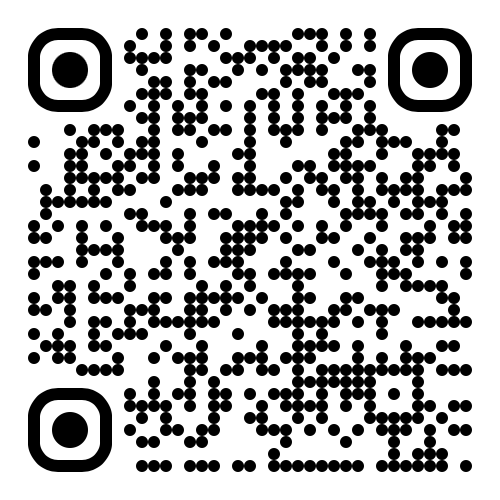
\includegraphics[width=0.5\linewidth]{ANNOY_github_black.png}
    \end{figure}
\centering
\small \href{https://github.com/ColZoel/Annoy_text_classifier}{https://github.com/ColZoel/Annoy\_text\_classifier}
\end{frame}


% Outline Slide
\begin{frame}{Outline}
    \tableofcontents
\end{frame}


\section{Introduction}

\begin{frame}{Problem Space}
    Input: 500 million to 1.3 billion unser-generated occupation titles
    \\Output: 969 O*Net classifications from Dingle
    \\Objective: map each title to a class with high accuracy
\end{frame}

\begin{frame}{Naive Solution}
    \begin{itemize}
        \item LLM prompt-based approach\\
        System role: You are an expert in text classification. \\Only output the answer. Use this list: $<[list]>$\\
        Prompt: Which item is this string most similar to? \\$<string>$
        \begin{itemize}
            \item Used in some NLP frameworks, such as SpaCy
            \item pairwise similarity $O(nm)$ time
            \item black box: results change dramatically between models
            \item Probabilistic: no guarantee of replicable results with the same model 
        \end{itemize}
    \end{itemize}
\end{frame}

\begin{frame}{Embedding-Based Solutions}
    \begin{itemize}
        \item Embedding + Cosine Similarity
        \\Find the label that maximizes the cosine similarity with the input
        \begin{align*}
            C(A,B) &= \cos(\theta) = \frac{A \cdot B}{\|A\| \|B\|}\\
            Y_{\text{best}} &= \arg\max_B C(A,B) 
        \end{align*}
        \begin{itemize}
            \item $Y \in [-1,1]$. 1 is perfect similarity
            \item pairwise similarity: $O(nm)$ time 
        \end{itemize}
    \end{itemize}
\end{frame}


\begin{frame}{Embedding-Based Solutions}
    \begin{itemize}
        \item Embedding + Neural Networks
        \\Find the label that maximizes the softmax in the output layer (most likely class)
        \\for a learned function $f: x \mapsto y $, 
        \begin{align*}
            Y_{best} = \arg\max (\text{softmax}(f(x)))
        \end{align*}
        \begin{itemize}
            \item $O(L \cdot M)$ time ($L=$ Layers, $M=$ neurons per layer)
            \item supervised: requires labeled data to train
            \item Embeddings are optimized for classification, not just semantic similarity
        \end{itemize}
    \end{itemize}
\end{frame}


\begin{frame}{Embedding-Based Solutions}
    \begin{itemize}
        \item Embedding + Clustering
        \\Find the label with the closest embeddings, which often share semantic similarities depending on the embedding structure.
        \\for a learned function $f: x \mapsto y $, where $c$ is a cluster centroid, 
        \begin{align*}
           Y_{best} = \arg\min_{c} \text{dist}(f(x), c)
        \end{align*}
        \begin{itemize}
            \item Approx. $O(N)$ time for naive search, faster with optimized structures (like ANN)
            \item For K-means: $O(NkT)$ time ($N$ = data points, $k$ = clusters, $T$ = iterations)
            \item unsupervised: no labels in training, used in prediction
            \item Close embeddings are classified similarly 
        \end{itemize}
    \end{itemize}
\end{frame}




\begin{frame}{Transformer}
Machine Learning technique for NLP based on the idea of "attention"
\begin{itemize}
    \item token-based: roots, prefixes, suffixes, words
    \item encodes word order
    \item attention encodes relationships across the entirety of a sentence
    \item capable of picking up nuances, e.g.
    \begin{center}
        Doctor Lawyer\\
        vs.\\
        Lawyer Doctor
    \end{center}
\end{itemize}
\end{frame}

\begin{frame}{Transformer}
\begin{figure}
    \centering
    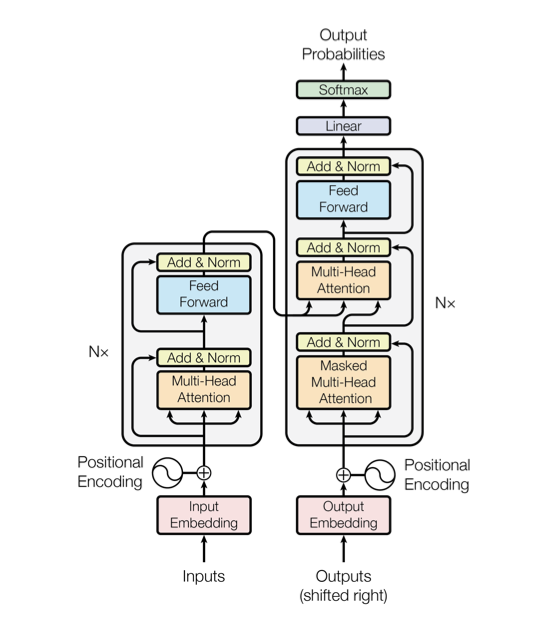
\includegraphics[width=0.5\linewidth]{images/architecture.png}
    \label{fig:enter-label}
\end{figure}

\end{frame}

\begin{frame}{LLM vs SLM}
    Large Language Model (LLM)
    \begin{itemize}
        \item 100s of billions or trillions of parameters
        \item designed for autoregressive models
        \item outputs a probabilistic decoding (text, image, etc.)
        \item GPT, LlaMa
    \end{itemize}
     Small Language Model (SLM)
    \begin{itemize}
        \item 100s of millions of parameters
        \item designed for encoder models
        string
        \item outputs numeric encoding of text
        \item distilaBERT, MiniLM
    \end{itemize}
   
\end{frame}


\begin{frame}{Setfit}
\begin{itemize}
    \item SLM built over older versions MiniLM 
    \item intended for fine-tuning
    \item few-shot learning: requires some examples for tuning (not optimal for highly noisy space)
    \item Does not return similarities
\end{itemize}
\end{frame}


\begin{frame}{Encoder Embeddings} 
    
    \begin{figure}
       \centering
        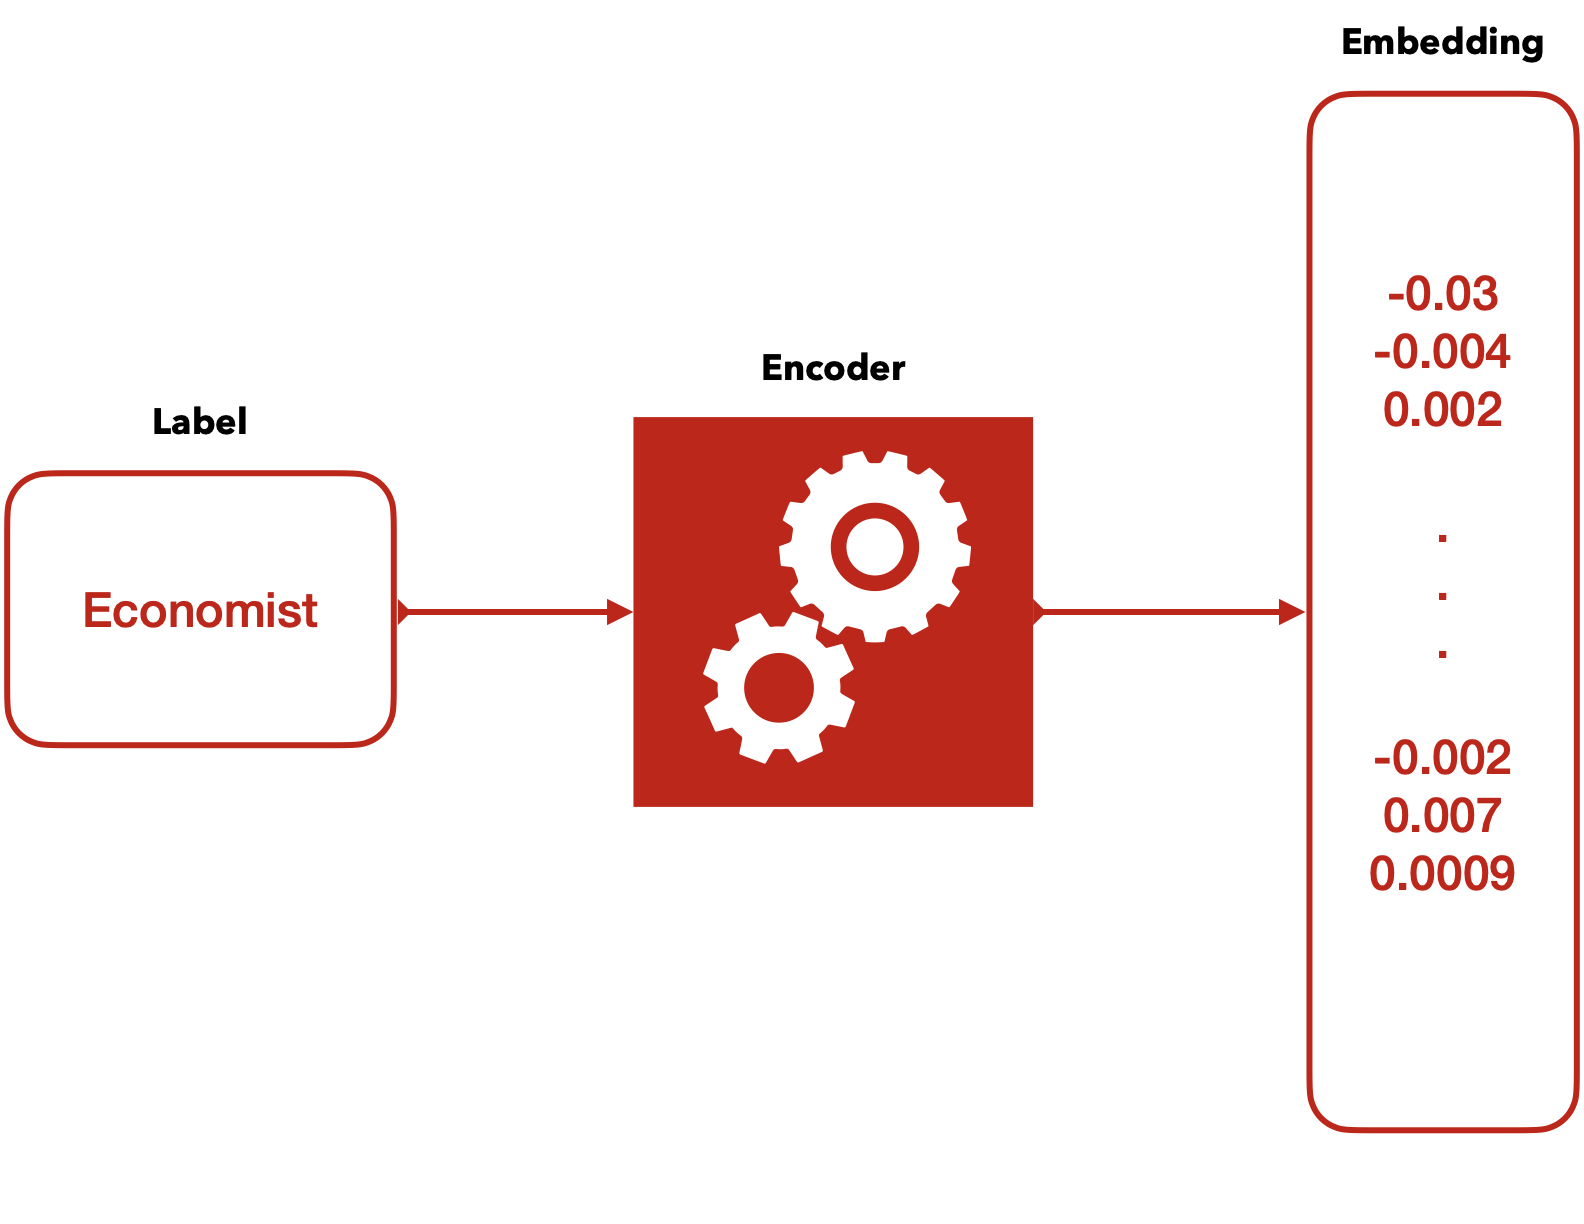
\includegraphics[width=.8\linewidth]{images/encoder.jpeg}
        \label{fig:encode}
    \end{figure}
    \vfill
\end{frame}




\section{ANN}
\begin{frame}{Approximate Nearest Neighbor}
\begin{itemize}
    \item General class of Nearest Neighbor search that looks for a ``good enough" path, rather than ``the best" path. 
    \item Search and partition optimizations 
    \item generally faster (but slightly less accurate) than other approaches

\end{itemize}
\end{frame}


\begin{frame}{Approximate Nearest Neighbor}
    \scriptsize
\begin{table}[h]

    \centering
    \renewcommand{\arraystretch}{1.3} % Slightly reduce row spacing
    \resizebox{\textwidth}{!}{
    \begin{tabular}{l|l|l}
        \toprule
        \textbf{Feature} & \textbf{ANN Methods} & \textbf{Clustering Methods} \\
        \midrule
        \textbf{Objective} & Find closest points quickly & Group data into meaningful clusters \\
        \textbf{Granularity} & Works at the \textbf{point} level & Works at the \textbf{group} level \\
        \textbf{Data Structure} & Uses \textbf{trees or graphs} & Uses \textbf{centroids, density, or hierarchy} \\
        \textbf{Focus} & Speed \& efficiency & Identifying data patterns \\
        \textbf{Handling New Data} & Often supports \textbf{incremental updates} & Requires \textbf{recomputing clusters} \\
        \textbf{High-Dimensionality} & More optimized (sublinear time) & May struggle with dense spaces (linear+ time) \\
        \bottomrule
    \end{tabular}
    }
    \caption{ ANN vs. Clustering}
    \label{tab:ann_vs_clustering}
\end{table}
\end{frame}


\begin{frame}{The ANN Family}
    \scriptsize
    \begin{table}[h]
    \centering
    \renewcommand{\arraystretch}{1.3} % Adjust row height for better readability
    \resizebox{\textwidth}{!}{
    \begin{tabular}{l|l|l}
        \toprule
        \textbf{ANN Method}          & \textbf{Partitioning Approach} & \textbf{Data Structure} \\
        \midrule
        \textbf{KD-Trees}            & Axis-aligned hyperplane splits & Binary trees \\
        \textbf{Randomized KD-Trees} & Random hyperplane splits & Multiple kd-trees \\
        \textbf{ANNOY}               & Random projections & Multiple random trees \\
        \textbf{HNSW} (Hierarchical Navigable Small World) & Graph-based layers of connections & Small-world graph \\
        \textbf{LSH}  (Locality-Sensitive Hashing) & Hashing points into buckets & Hash tables \\
        \bottomrule
    \end{tabular}
    }
    \caption{Common ANN Models}
    \label{tab:ann_data_structures}
\end{table}
\end{frame}


\begin{frame}{The ANN Family}
\begin{table}[h]
    \centering
    \renewcommand{\arraystretch}{1.1} % Slightly reduce row spacing
    \resizebox{\textwidth}{!}{ % Auto-scale to fit width
        \begin{tabular}{l|l|l|l|l}
            \toprule
            \textbf{Feature} & \textbf{ANNOY} & \textbf{KD-Trees} & \textbf{HNSW} & \textbf{LSH} \\
            \midrule
            \textbf{Partitioning} & Random hyperplanes & Axis-aligned splits & Graph-based & Hash-based \\
            \textbf{Data Structure} & Multiple trees & Single tree & Layered graph & Hash tables \\
            \textbf{Query Complexity} & Sublinear & Logarithmic & Sublinear & Constant-time lookup \\
            \textbf{Storage} & Can store on disk & Must fit in RAM & Must fit in RAM & Low-memory \\
            \textbf{Best for} & Large-scale vector search & Low-dimensional data & High accuracy & Fast lookups \\
            \bottomrule
        \end{tabular}
    }
    \caption{\scriptsize Comparison of ANN Methods}
    \label{tab:ann_comparison}
\end{table}
\end{frame}





\begin{frame}{ANNOY}
A special class of ANN that 
\end{frame}

\begin{frame}{ANNOY}
\begin{table}[h]
    \centering
    \renewcommand{\arraystretch}{1.3} % Adjust row height for better readability
    \resizebox{\textwidth}{!}{
    \begin{tabular}{l|l|l}
        \toprule
        \textbf{Feature} & \textbf{k-NN (Brute Force)} & \textbf{ANNOY (Approximate)} \\
        \midrule
        \textbf{Indexing Structure} & No index, direct distance calculations & Multiple random projection trees \\
        \textbf{Partitioning} & None & Recursive splitting via random hyperplanes \\
        \textbf{Search Method} & Exhaustive DFS & Priority queue-based backtracking \\
        \textbf{Query Speed} & (O(N)) & sublinear, $\sim O(\log N)$) \\
        \textbf{Scalability} & Bad for large datasets & Scales well to millions of points \\
        \textbf{Accuracy} & Exact & Approximate (but tunable) \\
        \bottomrule
    \end{tabular}
    }
    \caption{KNN vs. ANNOY}
    \label{tab:ann_vs_knn}
\end{table}
\end{frame}



\section{Methodology}


\begin{frame}{Methodology}
Embeddings + ANN Efficient Clustering
\begin{itemize}
    \item Embeddings for semantic representation
    \item cluster to find semantically similar strings
    \item Efficient for large data. Sublinear time: $O(log(n))$
\end{itemize}
\end{frame}


\begin{frame}{Process}
    \begin{enumerate}
        \item Embed labels (969 output classes)
        \item Build tree index with $ \Tau$ trees on embeddings 
        \item clean/standardize input (ASCII, alpha-numeric)
        \item embed input strings 
        \item query $n$ closest neighbors from forest
        \item majority vote for class label
    \end{enumerate}
\end{frame}




\begin{frame}{Train/Classify Mechanism}

    \begin{figure}
       \centering
        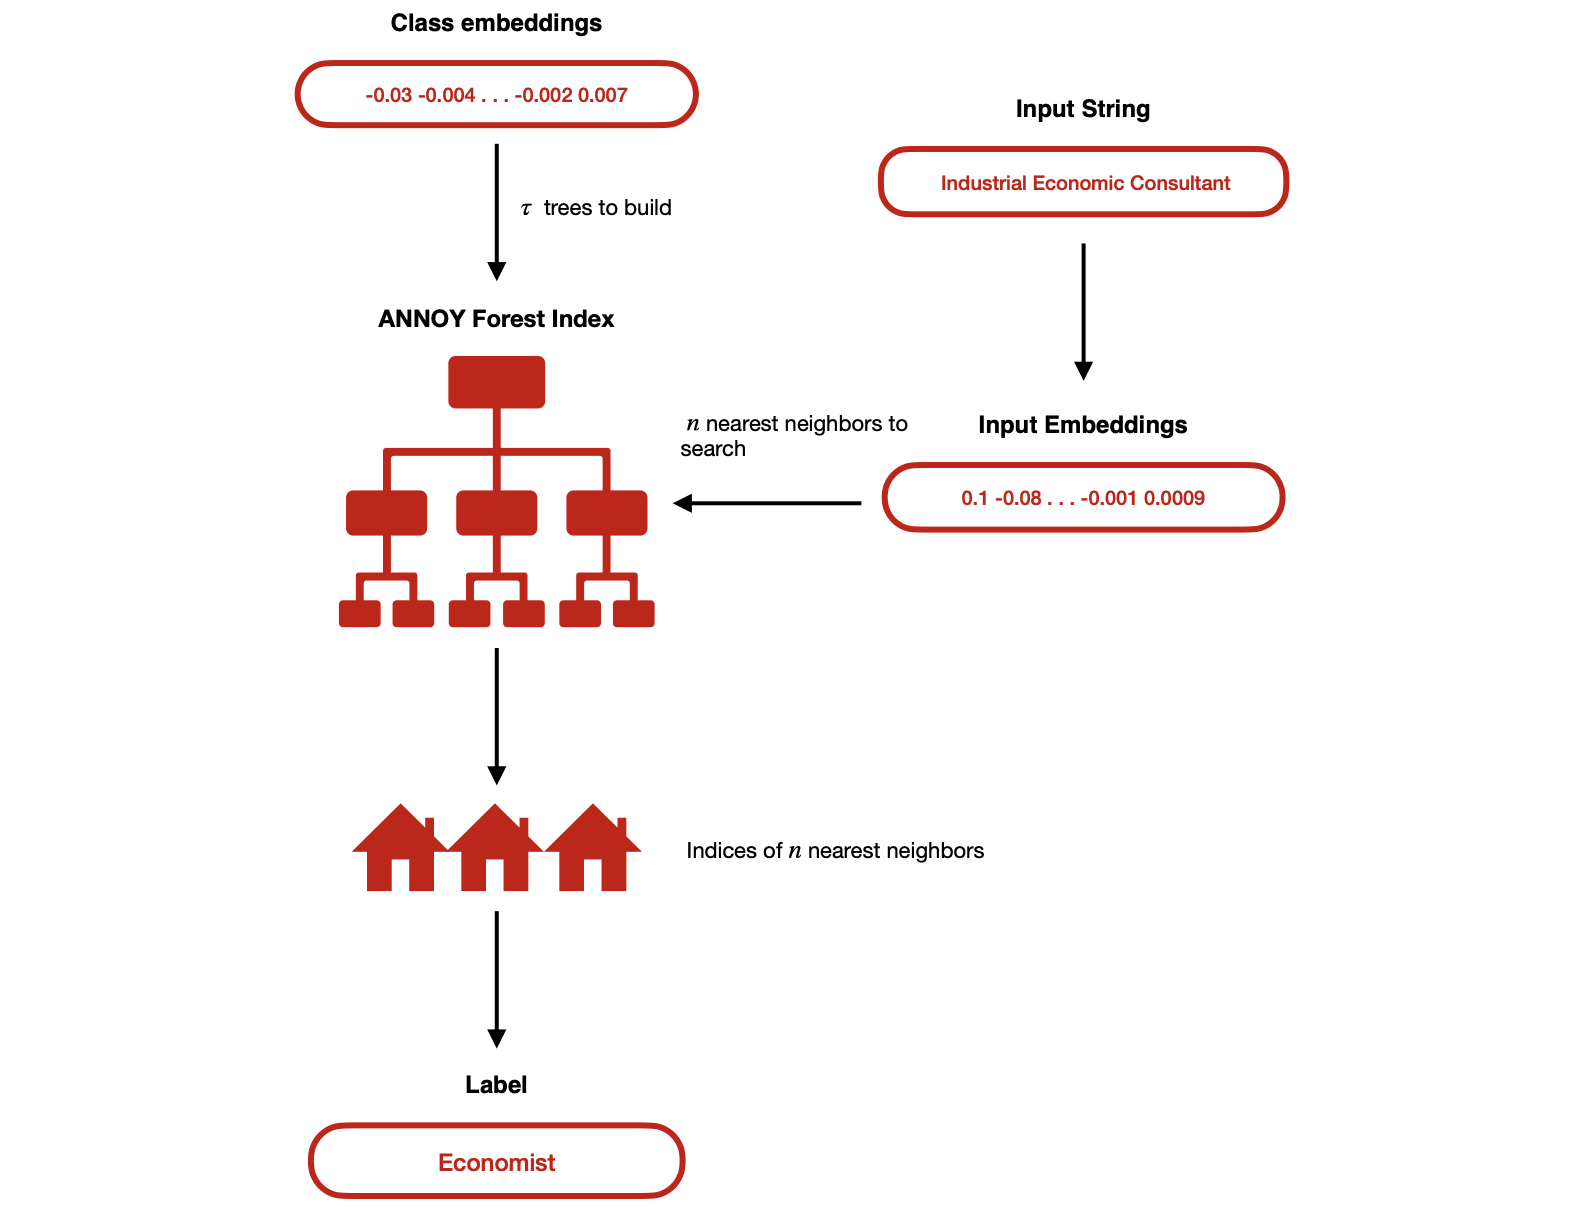
\includegraphics[width=.75\linewidth]{images/pipe.jpeg}
        \label{fig:pipe}
    \end{figure}
    \hfill
\end{frame}

\section{Sandbox Results}

\begin{frame}{Data}
1.5 million observations of job titles scraped from Linked, Indeed, and other sources. Obtained from Kaggle and an independent researcher (from Reddit)
\end{frame}

\begin{frame}{Small Sample $n=100$,  $k=1$ and $\Tau=5000$}
    \begin{figure}
        
        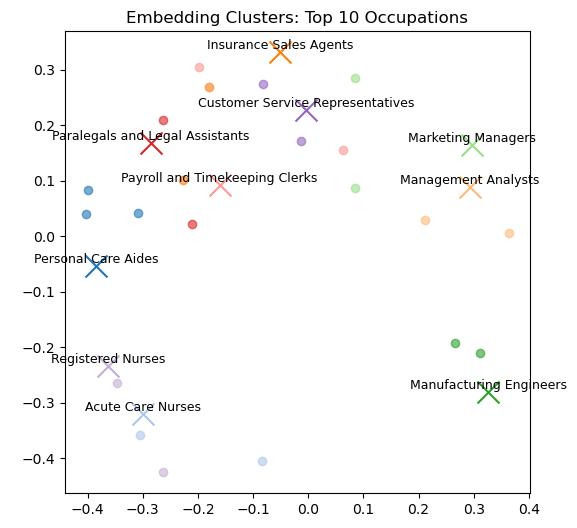
\includegraphics[width=0.6\linewidth]{images/100_small_samples.png}
        \label{fig:k1t1000}
    \end{figure}
\end{frame}



\end{document}